\subsection{Why partial least squares structural equation modelling}
\label{model:why-plssem}

We use partial least squares structural equation modelling (PLS-SEM,
R package \texttt{seminr} \citep{Rseminr}) to estimate the full structural model in one
step. PLS-SEM was chosen for three reasons specific to this data. First, it
accommodates formative and reflective constructs simultaneously within a
single estimation: tolerance is reflective (Section~\ref{measurement:tolerance}),
while conflict experience, tangible cost, intangible cost, compensation
anticipation, and policy support are formative
(Section~\ref{measurement:formative}). Second, it does not require
multivariate normality, which is convenient given the skewed monetary
variables described in Section~\ref{data:quality}. Third, it remains reliable
at our sample size ($n = 625$) with a comparatively complex construct
structure.

\subsection{Model specification}
\label{model:spec}

The structural model links four layers of constructs: a background layer
(conflict experience with wild boar and with all species, survey site,
national-park residence, and sociodemographics -- gender, age, education,
income, household assets); an exposure layer (prevention effectiveness and
compensation participation, CE0); a mediator layer (compensation
anticipation, policy support, tangible cost, intangible cost, and intangible
benefit); and the outcome, tolerance. Every construct in an earlier layer has
a direct structural path to every construct in a later layer, including a
direct path from each background variable to tolerance itself; this dense
specification is what lets us report, for example, that a given
predictor's effect on tolerance is estimated \emph{after} already accounting
for site, national-park residence, and demographics in the same equation,
rather than as a separate, unadjusted comparison. Skewed monetary indicators
enter log-transformed within their formative blocks, exactly as in
Section~\ref{measurement:features}. All paths are estimated jointly and
bootstrapped with 5{,}000 resamples to obtain standard errors and $p$-values
for every path simultaneously. Because the underlying data are
cross-sectional and observational, every coefficient below should be read as
an \emph{association}, adjusted for the other variables in the same model,
not as a causal effect.

\subsection{RQ1: does compensation predict tolerance, and is the effect mediated?}
\label{model:rq1}

The full model explains a meaningful share of the variance in tolerance
($R^2 = 0.234$), driven predominantly by intangible cost and, to a lesser
extent, intangible benefit and prevention effectiveness. Table~\ref{tab:rq1}
reports the four direct predictors with a significant path to tolerance.

\begin{table}[htbp]
\centering
\caption{Direct predictors of tolerance with a significant path in the full
structural model ($R^2 = 0.234$; $n = 625$; 5{,}000 bootstrap resamples).}
\label{tab:rq1}
\begin{tabular}{lrr}
\hline
\textbf{Predictor} & \textbf{$\beta$} & \textbf{$p$} \\
\hline
Intangible cost (IC)              & $-0.34$  & $<.001$ \\
Intangible benefit (IB)           & $+0.16$  & $<.001$ \\
Prevention effectiveness (PE)     & $+0.11$  & .005 \\
Compensation participation (CE0)  & $-0.109$ & .003 \\
\hline
\end{tabular}
\end{table}

\begin{figure}[htbp]
\centering
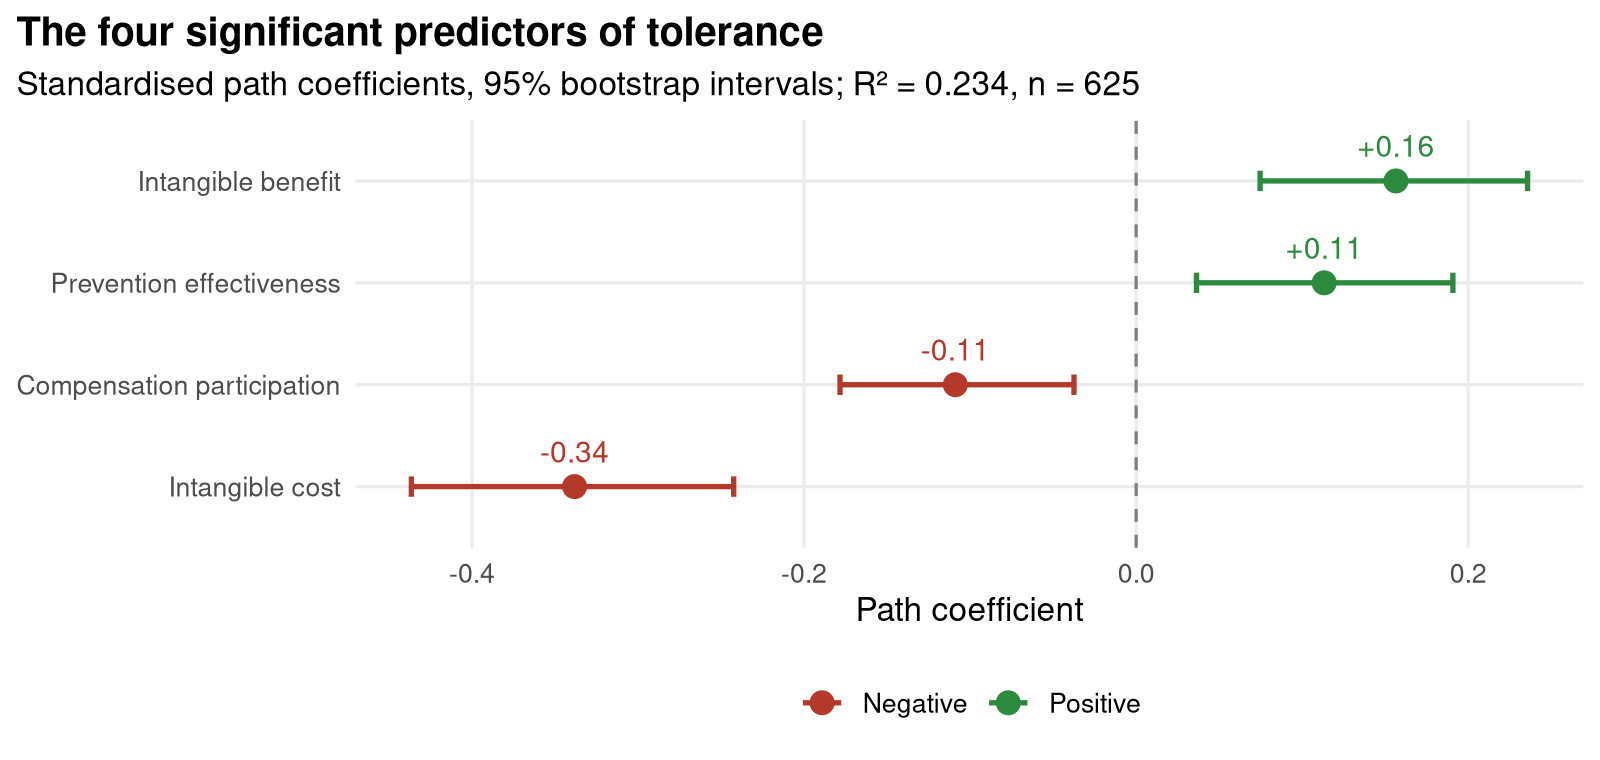
\includegraphics[width=0.8\textwidth]{figures/fig_rq1_paths.png}
\caption{Standardized path coefficients from the four significant direct
predictors of tolerance, with 95\% bootstrap intervals. Red: negative
association; green: positive association.}
\label{fig:rq1-paths}
\end{figure}

\begin{figure}[htbp]
\centering
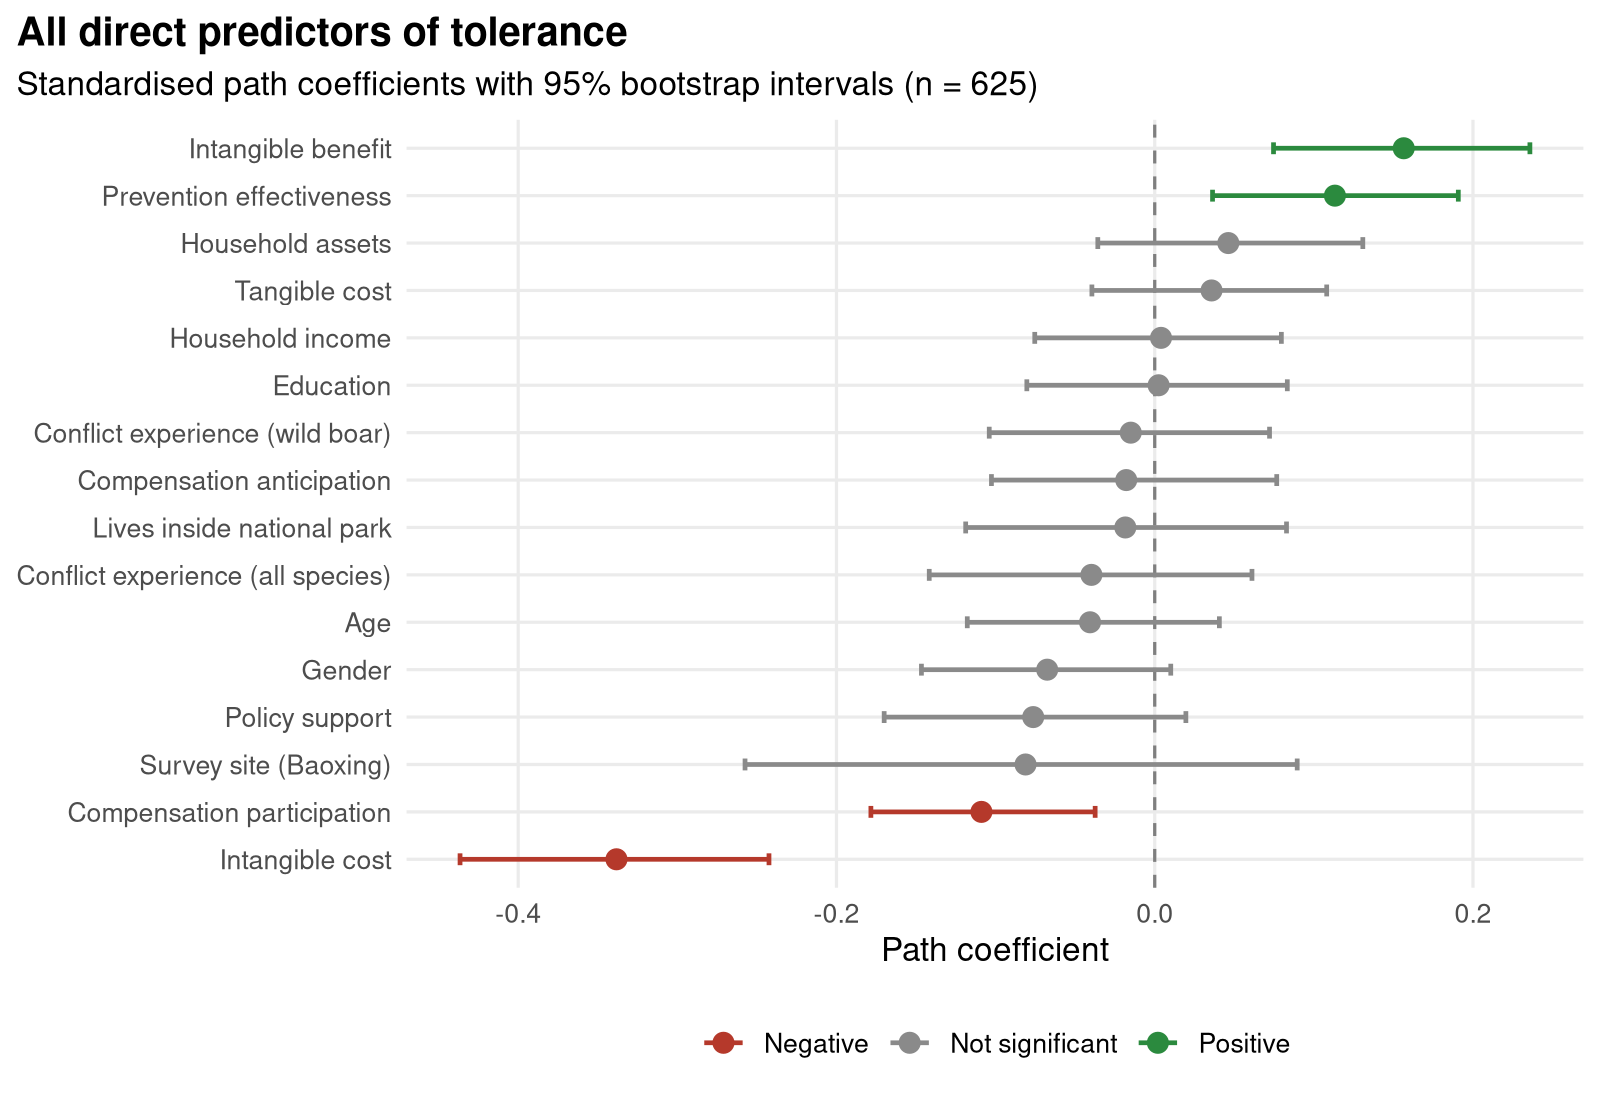
\includegraphics[width=0.85\textwidth]{figures/fig_all_direct_paths.png}
\caption{All direct paths to tolerance in the full structural model, with
95\% bootstrap intervals. Green: positive; red: negative; grey: interval
includes zero.}
\label{fig:all-paths}
\end{figure}

Figure~\ref{fig:rq1-paths} shows all four paths together; Figure~\ref{fig:all-paths}
shows every direct path to tolerance in the model, including those that
are not significant. Intangible cost has the strongest association with tolerance of any
predictor in the model ($\beta = -0.34$, $p < .001$): residents who perceive
more intangible cost from wild boar report markedly lower tolerance.
Intangible benefit ($\beta = +0.16$, $p < .001$) and prevention effectiveness
($\beta = +0.11$, $p = .005$) both associate positively with tolerance.
Compensation participation itself has a smaller, but still significant,
negative association with tolerance ($\beta = -0.109$, $p = .003$), even
after adjusting for survey site -- we refer to this as the
\emph{compensation paradox} throughout this report, since it runs opposite
to the policy assumption that compensation should raise tolerance.

A conceptual point is worth stating clearly before going further, because
the next result can otherwise look like it contradicts the one just given.
Section~\ref{model:rq1} above already established that compensation
participation has a real, statistically robust association with tolerance
(Table~\ref{tab:rq1}; and, as Section~\ref{robustness} shows, that association
is negative in all 8{,}192 alternative model specifications we tested). That
is one question -- \emph{does} compensation participation associate with
tolerance? -- and it has a clear answer: yes. Mediation analysis asks a
second, logically separate question: \emph{through which of our measured
variables} does that association travel? An effect can be real, large, and
completely robust while none of a specific, finite list of candidate
mediators explains it -- this happens whenever the true mechanism runs
through something the study did not measure. Finding no significant
mediator among the five we tested therefore does not weaken or cast doubt on
the direct effect established above; it means only that this particular
analysis cannot yet say \emph{why} the effect exists, which is precisely the
open question this subsection reports.

With that distinction in mind: we tested whether the compensation--tolerance
association runs through the five measured mediator constructs
(compensation anticipation, policy support, tangible cost, intangible cost,
and intangible benefit), using bootstrapped specific-indirect-effect tests
\citep{Nitzl2016}. Table~\ref{tab:mediation} reports the result: none of the
five specific indirect paths is individually significant (all $p > .16$),
and the total indirect effect summed across all five is small ($-0.024$),
corresponding to a variance-accounted-for (VAF) of 18\% of the total
compensation--tolerance association.

\begin{table}[htbp]
\centering
\caption{Bootstrapped specific-indirect-effect tests for compensation
participation $\rightarrow$ mediator $\rightarrow$ tolerance
\citep{Nitzl2016}, with 95\% percentile bootstrap confidence intervals.
Direct effect: $-0.109$ ($p=.003$). Total indirect effect: $-0.024$
(VAF $=18\%$).}
\label{tab:mediation}
\begin{tabular}{llrrrr}
\hline
\textbf{Code} & \textbf{Construct} & \textbf{Indirect effect} & \textbf{SE} & \textbf{95\% CI} & \textbf{$p$} \\
\hline
CA & Compensation anticipation & $-0.0017$ & 0.0046 & $[-0.010,\ 0.009]$ & .800 \\
PS & Policy support            & $-0.0013$ & 0.0054 & $[-0.013,\ 0.010]$ & .808 \\
TC & Tangible cost             & $+0.0027$ & 0.0036 & $[-0.003,\ 0.011]$ & .382 \\
IC & Intangible cost           & $-0.0178$ & 0.0141 & $[-0.048,\ 0.008]$ & .165 \\
IB & Intangible benefit        & $-0.0060$ & 0.0070 & $[-0.021,\ 0.007]$ & .354 \\
\hline
\end{tabular}
\end{table}

In other words, most
of the compensation paradox is not explained by the mediators we measured.
The confidence intervals show how strong this statement is. A
non-significant indirect effect is an absence of evidence, not evidence of
absence: the interval for intangible cost, the most plausible mediator, runs
from $-0.048$ to $+0.008$, so an indirect path of up to roughly 40\% of the
direct effect remains compatible with the data. With a bootstrap standard
error of 0.014, this design would detect an indirect effect through
intangible cost with 80\% power only if it were about 0.04 or larger. The
other four intervals are much tighter around zero. So this does not mean
there is no mechanism connecting compensation to tolerance. Two explanations
remain open. The mechanism may run through
something outside this measurement model: unmeasured grievance related to the
compensation process, prior conflict history not captured by our conflict-
experience items, or some other shared cause behind both compensation-seeking
and lower tolerance. Alternatively, the mediators may be measured too
noisily to carry the effect they really transmit; we examine this second
possibility in Section~\ref{discussion:sensitivity}. This is an open question for future data collection
(Section~\ref{discussion}), not a settled mechanism.

Why do the cost constructs, which the Wildlife Tolerance Model places between
compensation and tolerance, not act as mediators here? An indirect effect is
the product of two legs: compensation must predict the mediator, and the
mediator must predict tolerance. Figure~\ref{fig:mediation-legs} shows both
legs for each construct. Intangible cost and intangible benefit clearly
predict tolerance (second leg), but compensation participation does not
predict either of them once county, conflict experience, and demographics
are adjusted for (first leg: $+0.05$ and $-0.04$, both intervals include zero).
Tangible cost fails on both legs: applicants report somewhat more damage
($+0.07$, not significant), and damage is unrelated to tolerance ($+0.04$).
In plain terms, applicants and non-applicants perceive similar costs and
benefits of wild boar, so those perceptions cannot be what makes applicants
less tolerant. The same logic explains the absence of moderation in
Section~\ref{model:rq2}: costs and benefits relate to tolerance in the same
way in both groups.

\begin{figure}[htbp]
\centering
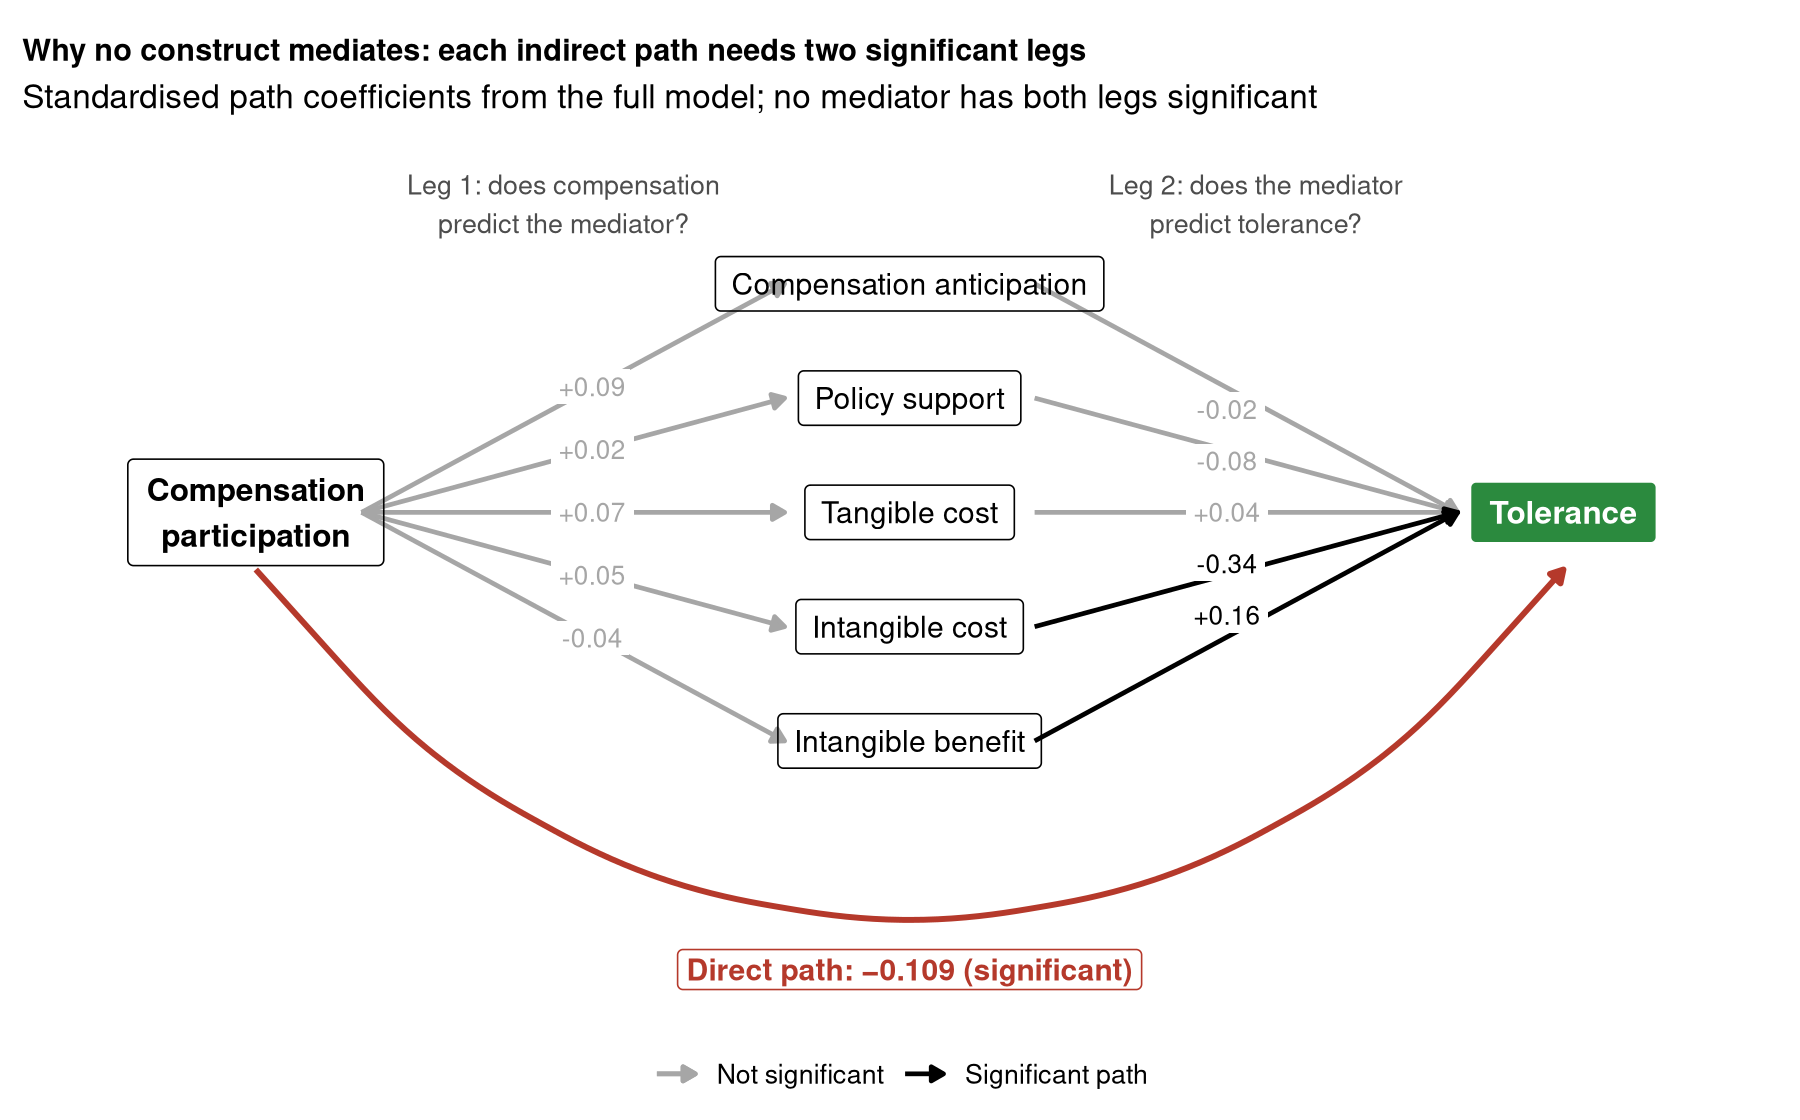
\includegraphics[width=0.95\textwidth]{figures/fig_mediation_legs.png}
\caption{The two legs of each indirect path from compensation participation
to tolerance. Black arrows: 95\% bootstrap interval excludes zero; grey:
includes zero. No construct has two black legs.}
\label{fig:mediation-legs}
\end{figure}

\begin{figure}[htbp]
\centering
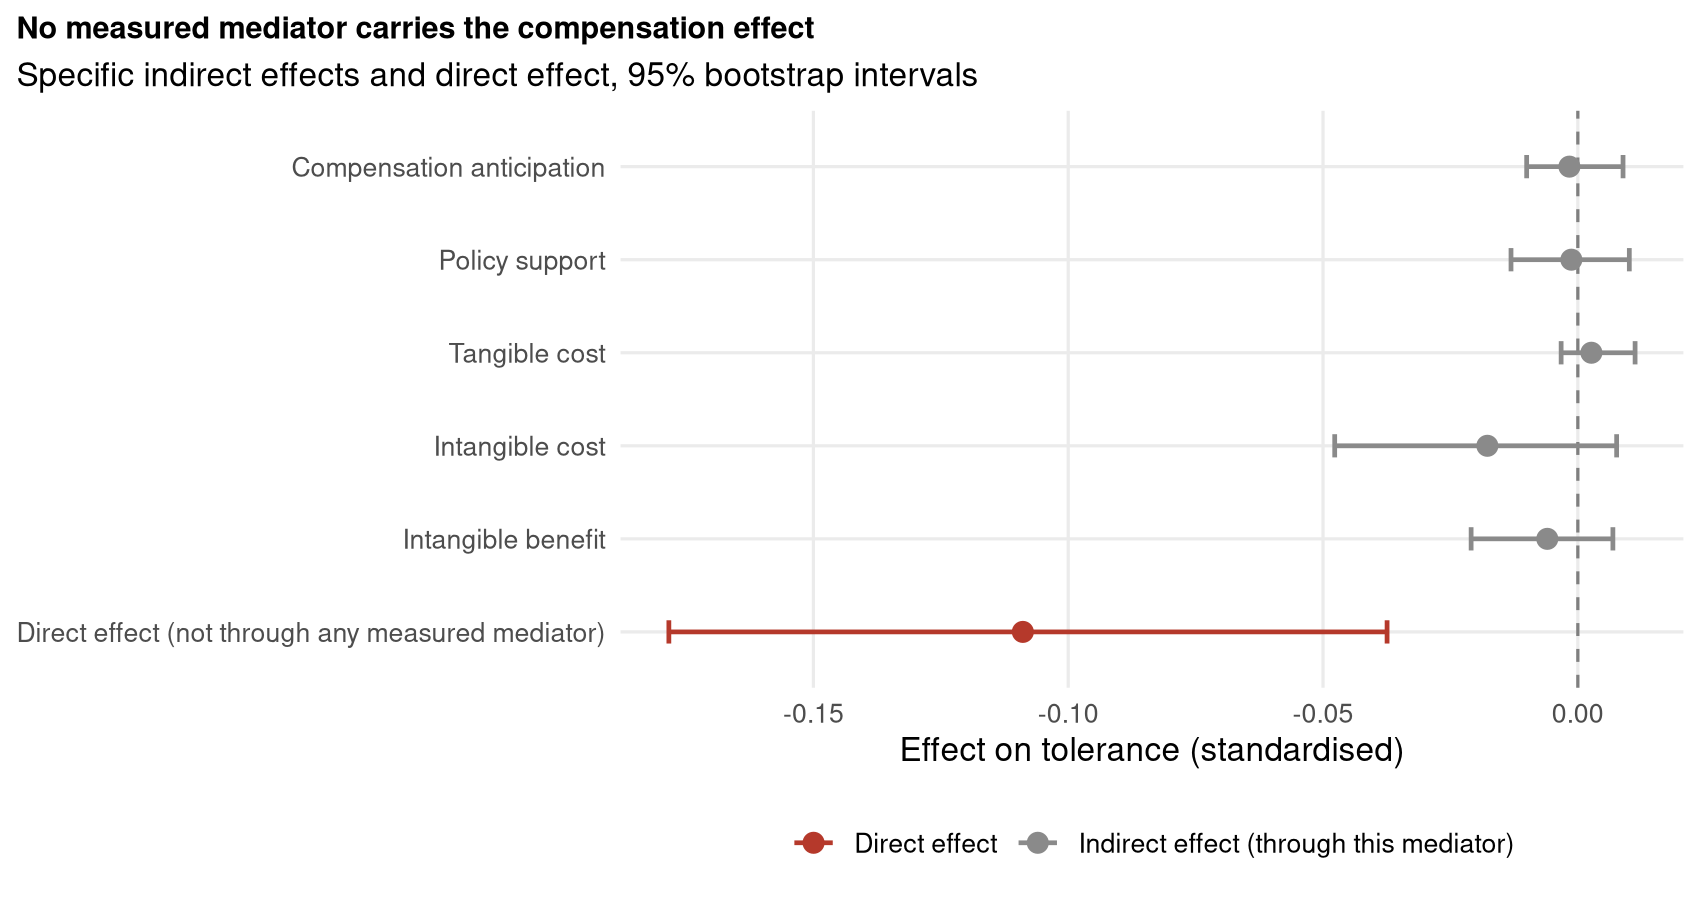
\includegraphics[width=0.9\textwidth]{figures/fig_mediation.png}
\caption{Specific indirect effects of compensation participation on
tolerance (grey) and the direct effect (red), with 95\% bootstrap intervals.
All five indirect intervals include zero; the direct effect does not.}
\label{fig:mediation}
\end{figure}

\subsection{Model checks on individual paths}
\label{model:checks}

Three additional checks qualify how confidently individual paths above
should be read. First, as already noted in Section~\ref{measurement:tolerance},
tolerance's reliability, while improved by dropping Tol3, still falls short
of the conventional threshold by the $\alpha$ and $\rho_A$ criteria; treat
tolerance throughout as a meaningful but noisy measure. Second, policy
support overlaps empirically with conflict experience and with survey site:
HTMT is 1.01 against conflict experience and 1.22 against site, both above
the 1.0 ceiling that normally signals a discriminant-validity problem. The two conflict-experience constructs also overlap with each other (HTMT
1.17). HTMT was designed for reflective constructs, and here it is applied to
formative composites and single items, so these values are a warning sign
rather than a formal test. We
therefore do not build a strong substantive claim on the policy-support path
in isolation -- whatever that path's coefficient captures may be entangled
with conflict experience and site rather than policy support specifically.
Third, survey site significantly predicts all five mediator constructs
(policy support, tangible cost, intangible cost, and intangible benefit at
$p < .001$; compensation anticipation at $p = .044$), but has no significant
remaining direct path to tolerance once those mediators are in the model
($\beta = -0.08$, $p = .34$). We read this as reassuring rather than
concerning: site's entire detectable influence on tolerance appears to run
through the mediators already in the model, rather than through some
separate, unmodelled channel.

\subsection{RQ2: do costs and benefits work differently after compensation?}
\label{model:rq2}

RQ2 asks whether the relationships between costs/benefits and tolerance
change depending on compensation experience -- that is, whether compensation
\emph{moderates} these relationships. We tested this directly with three
interaction terms (compensation participation $\times$ tangible cost,
$\times$ intangible cost, and $\times$ intangible benefit) in a two-stage
moderation model, rather than by comparing separately-fitted coefficients in
each group. The interaction-term approach is the stronger test: comparing two
separately-estimated group coefficients only tells you the two numbers look
different, not whether that difference is statistically distinguishable from
sampling noise in two smaller subsamples; a formal interaction term tests the
difference in slopes directly, using the full sample in one joint estimation.

All three interactions are non-significant (tangible cost $\times$
compensation, $p = .216$; intangible cost $\times$ compensation, $p = .234$;
intangible benefit $\times$ compensation, $p = .899$). This first moderation
model contains only the three cost and benefit constructs, compensation
participation, and their interactions. Because compensation participation is
confounded with county (Section~\ref{data:confound}), we repeated the test
with the full control set of the main model in the tolerance equation
(survey site, national-park residence, both conflict-experience constructs,
demographics, prevention effectiveness, compensation anticipation, and policy
support). The conclusion is the same: $p = .312$, $.142$, and $.871$
respectively, with compensation participation itself still negative
($\beta = -0.106$, $p = .004$). An ordinary regression on observed scores
with the same controls agrees, both for the single interactions (all
$p > .31$) and for a joint test of all three ($F = 0.49$, $p = .69$). The cost/benefit
relationships with tolerance are the same strength regardless of
compensation status: intangible cost remains the strongest negative
predictor and intangible benefit remains positive in both groups, and
compensation experience does not alter either slope. Figure~\ref{fig:interaction-forest} plots the three interaction coefficients
with their intervals, for the model without and with controls: all include
zero. One exploratory observation qualifies this. If interactions of the
costs and benefits with \emph{county} are added to the observed-score
regression as well, the intangible cost $\times$ compensation term
($+0.21$, $p = .028$) and the intangible cost $\times$ county term ($-0.26$,
$p = .029$) both become nominally significant, with opposite signs. These
are two of six additional tests, they are not corrected for multiplicity, and
compensation and county are too entangled to separate cleanly in this way, so we
report it only as an indication that the strength of the intangible
cost--tolerance relationship may vary across settings, not as a finding. Figure~\ref{fig:slopes} shows the
same question informally, as fitted lines of tolerance against each predictor
separately for applicants and non-applicants. These raw lines are
unadjusted, so differences in their slopes (for instance for intangible
benefit) can reflect other differences between the groups; the adjusted
interaction tests in Figure~\ref{fig:interaction-forest} are the
formal answer.

\begin{figure}[htbp]
\centering
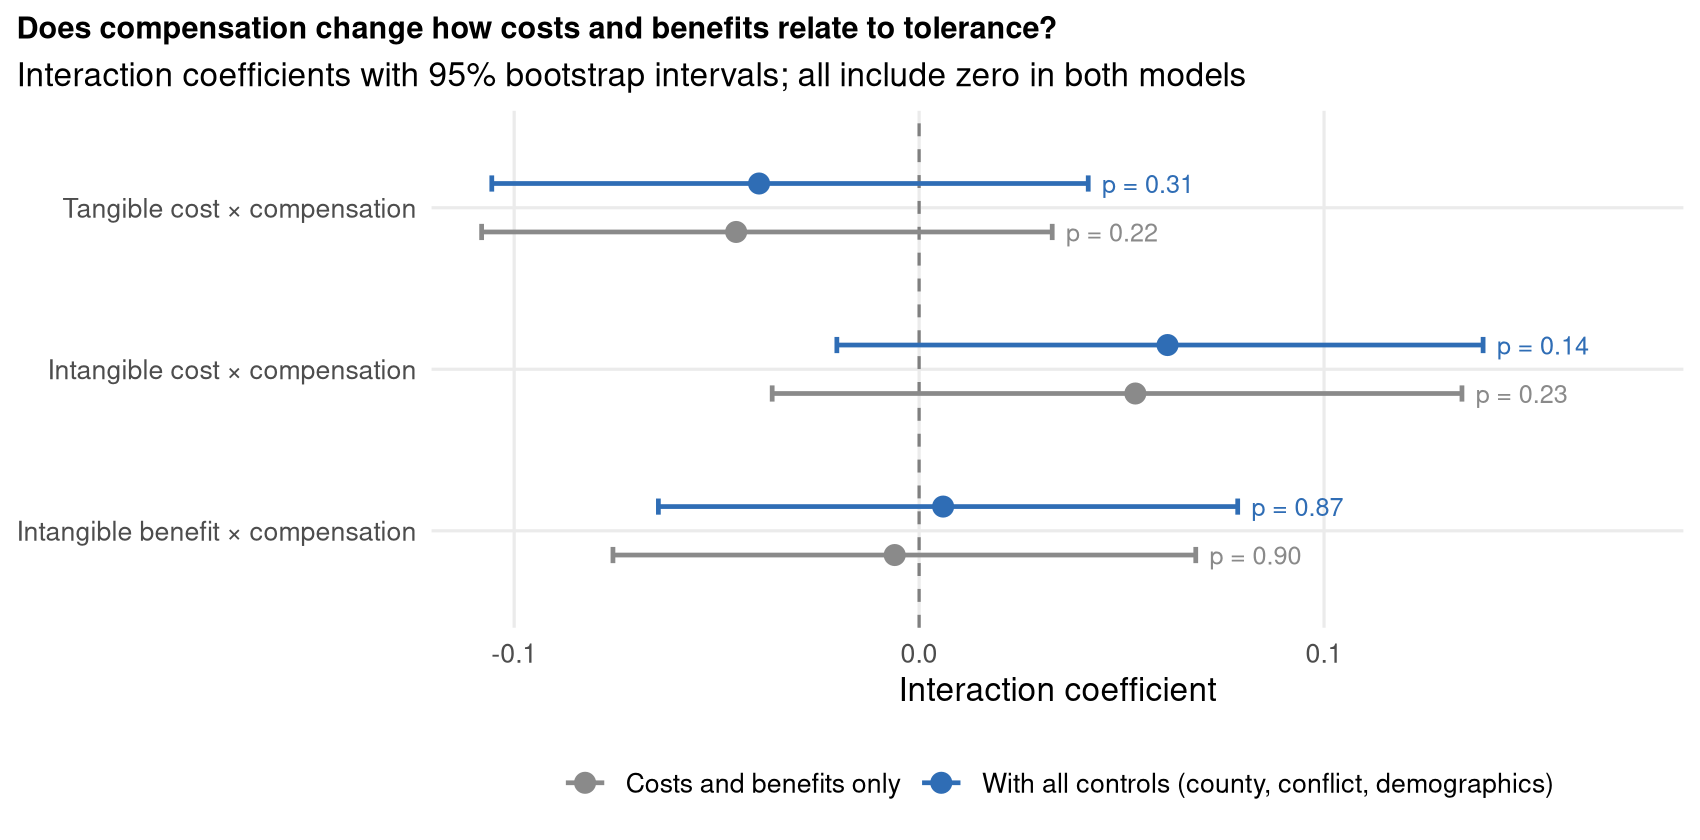
\includegraphics[width=0.9\textwidth]{figures/fig_interaction_forest.png}
\caption{Interaction coefficients (compensation participation $\times$
cost or benefit) on tolerance, with 95\% bootstrap intervals, from the
model with costs and benefits only (grey) and the model with the full
control set (blue).}
\label{fig:interaction-forest}
\end{figure}

\begin{figure}[htbp]
\centering
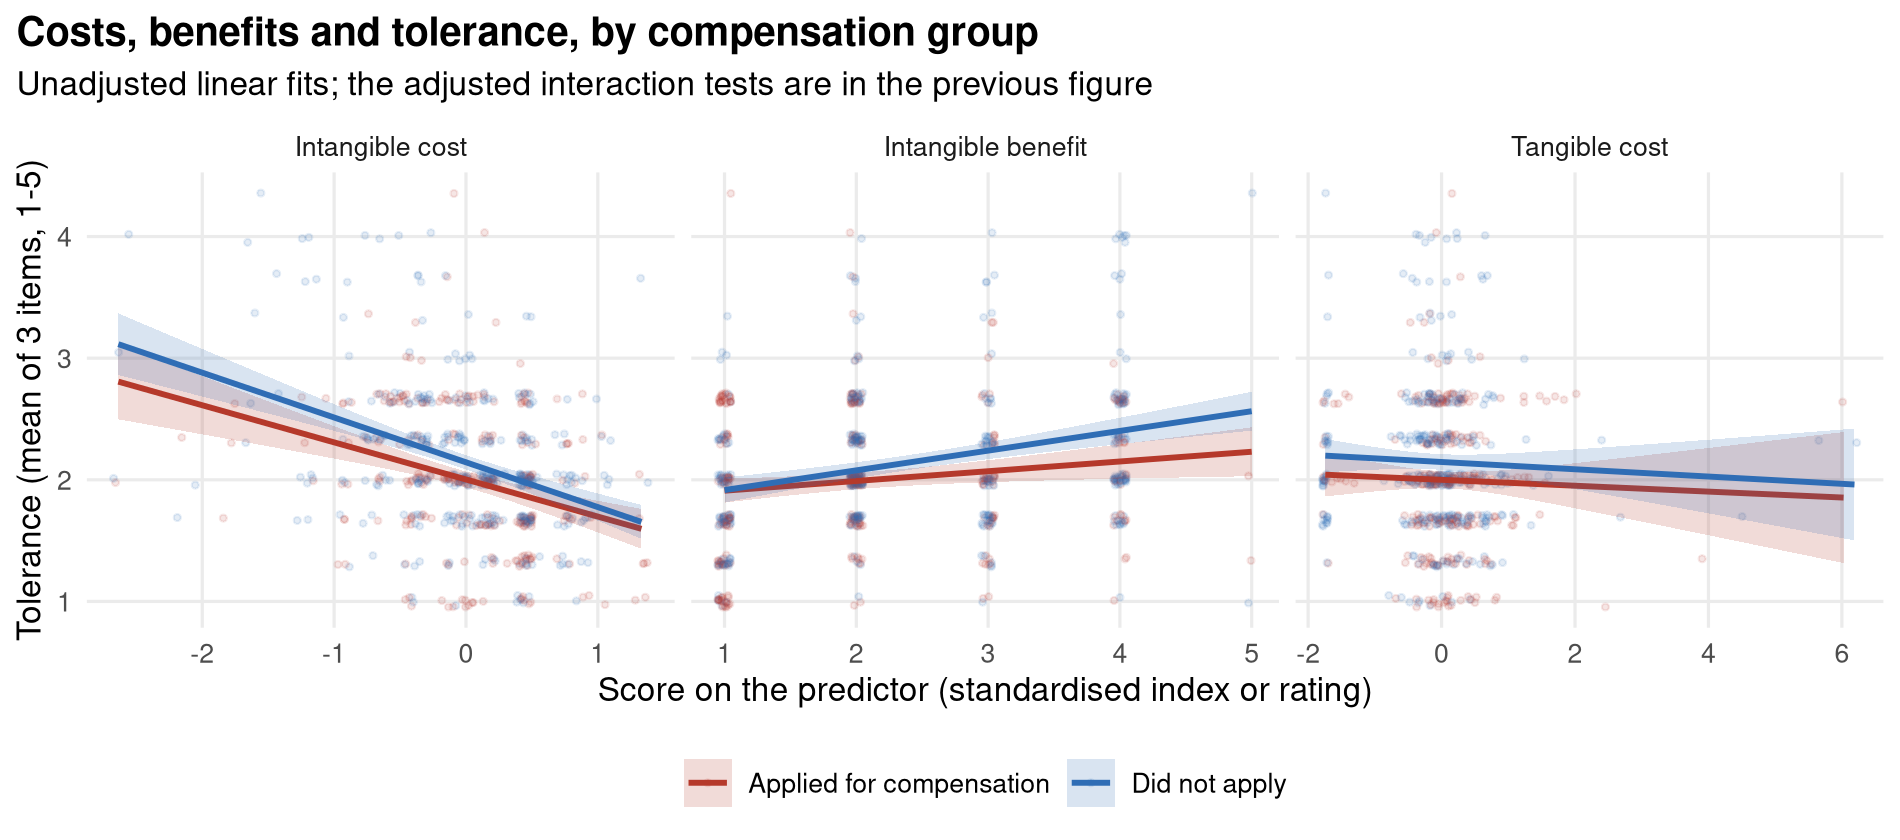
\includegraphics[width=\textwidth]{figures/fig_slopes_by_group.png}
\caption{Tolerance against intangible cost, intangible benefit, and
tangible cost, separately for households that did and did not apply for
compensation (unadjusted linear fits with 95\% confidence bands).}
\label{fig:slopes}
\end{figure}

\subsection{Summary of the main-analysis findings}
\label{model:summary}

For RQ1, compensation participation is negatively associated with tolerance,
and no specific measured mediator explains why. For RQ2, intangible cost is
the strongest negative predictor of tolerance and intangible benefit is a
positive one, and compensation status does not change the strength of
either relationship. Both findings are associations from a single
cross-sectional survey with an incomplete measurement model; they motivate
specific follow-up questions (Section~\ref{discussion}) rather than closing
the topic.

Table~\ref{tab:findings-count} counts what was and was not significant. The
original survey sheet has 57 columns. After removing the identifier, the
township and village labels, the four tolerance items (the outcome), and
the two applicant-only follow-up items, 48 variables remain as candidate
covariates (county enters as survey site). Screened one at a time
(Appendix~\ref{app:screen}), 15 are associated with tolerance at $p < .05$ and
10 after controlling the false discovery rate at 5\%; with county as an
additional covariate, 12 survive. These counts overstate the number of
independent findings, since five of the significant variables are
different indicators of the same construct (intangible cost) and several others
measure conflict with other species. In the full structural model, where the
variables are grouped into constructs and adjusted for each other, four
constructs are significantly associated with tolerance.

\begin{table}[htbp]
\centering
\caption{Summary of significant findings.}
\label{tab:findings-count}
\begin{tabular}{p{4.6cm}p{2.2cm}p{6.2cm}}
\hline
\textbf{Question} & \textbf{Count} & \textbf{Which} \\
\hline
Survey variables associated with tolerance, one at a time (of 48) & 15 nominal; 10 after FDR control & General attitude to wild boar and word ratings (intangible cost), ecological value (intangible benefit), prevention effectiveness, lowest accepted compensation, severity and duration of conflict with all species, potato area \\
Constructs with a significant direct path to tolerance (of 16) & 4 & Intangible cost ($-0.34$), intangible benefit ($+0.16$), prevention effectiveness ($+0.11$), compensation participation ($-0.109$) \\
Significant mediators of the compensation effect (of 5) & 0 & None; total indirect effect $-0.024$ (18\%) \\
Significant interactions with compensation (of 3) & 0 & None, without or with the full control set \\
Significant moderators & 0 in the interaction tests & Compensation status does not moderate any cost or benefit path; the multi-group analysis finds one exploratory difference (Section~\ref{robustness:mga}) \\
\hline
\end{tabular}
\end{table}
